% compile with XeLaTeX or LuaLaTeX
\documentclass[10pt,a5paper,twoside]{article}
\usepackage{iftex}
\RequireXeTeX
\usepackage[top=12mm,bottom=26mm,outer=28mm,inner=14mm,foot=14mm]{geometry}
\usepackage{calc}
\usepackage{scrextend}
\deffootnote[1.5em]{0em}{1em}{\thefootnotemark\quad}
\renewcommand{\footnoterule}{%
  \kern -2.4pt
  \hrule width \textwidth height 0.4pt
  \kern 2pt
}

\usepackage{fontspec}
\setmainfont[
	Ligatures=TeX,
	Extension=.otf,
	SlantedFont=cmunsl,
	BoldFont=cmunbx,
	ItalicFont=cmunti,
	BoldItalicFont=cmunbi,
	SmallCapsFont=cmunrm, % for upright instead of slanted small caps
	SmallCapsFeatures={Letters=SmallCaps,Numbers=OldStyle},	
]{cmunrm}

\usepackage{etoolbox}
\usepackage{microtype,ellipsis}

\usepackage{polyglossia,iflang}
\setotherlanguage{russian} % the name of the original Russian version at the end of this book is written using Cyrillic letters

\usepackage{textcomp}

\usepackage{amsmath,amssymb,nicefrac,amscd}
\usepackage{graphicx,float}
\usepackage{import}
\usepackage{pdfpages}

\usepackage{enumitem}
\setitemize[1]{noitemsep,nosep,leftmargin=0.99em,label={--}}

\usepackage{transparent}
\usepackage{csquotes}
\DeclareQuoteStyle{vietnamese}
  {\textquotedblleft}
  {\textquotedblright}
  [0.05em]
  {\textquoteleft}
  {\textquoteright}

\usepackage{siunitx}
\sisetup{per-mode=fraction,fraction-function=\nicefrac}

\usepackage{hyperref}

\usepackage{todonotes}

\newcommand{\eps}{\varepsilon}

% Usually, you would define a theorem-like enviroment which uses automatic numbering
% but Arnold also uses special numbering for some problems. Therefore, I kept the manual numbering.
\newenvironment{problem}[1]{\paragraph*{#1}}{}

\newenvironment{note}[1]{\par\noindent\IfLanguageName{vietnamese}{\textit{#1}}{\textsc{\MakeLowercase{#1}}} }{\par}

\makeatletter

% do no indent the first paragraph of the abstract
\let\oldabstract\abstract
\def\abstract{\oldabstract\noindent\@ifnextchar\par{\expandafter\abstract\@gobble}{}}

% always center contents of floats
\g@addto@macro\@floatboxreset{\centering}

% make all figures use 'H' position by default:
\def\fps@figure{H}
\makeatother

\setdefaultlanguage[babelshorthands = false]{italian}

\title{Problemi per ragazzini dai 5 ai 15 anni}

\author{V.\,I.~Arnold
\vspace*{2cm}\\
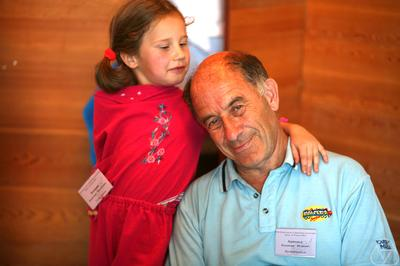
\includegraphics[width=\linewidth]{resources/photo-arnold_small}
}
\date{}

\begin{document}
\maketitle
\thispagestyle{empty}
\cleardoublepage
\setcounter{page}{1}
\begin{abstract}
Questo fascicolo presenta 77 problemi utili a sviluppare la capacità di ragionare, che l’autore ha scelto o ha composto di suo pugno. In generale, la loro soluzione non richiede conoscenze diverse da quelle che si acquistano in un abuona scuola secondaria. Ma per alcuni di essi, venirne a capo, può rivelarsi una sfida anche per molti professori.

Il libro si rivolge a studenti, universitari, insegnanti, genitori – a chiunque consideri la cultura del ragionamento una parte essenziale dello sviluppo della personalità.
\end{abstract}
\clearpage

\section*{Prefazione}
Ho messo questi problemi su carta a Parigi nella primavera del 2004, quando alcuni Russi residenti a Parigi mi chiesero di aiutare i loro ragazzi a recuperare la cultura del ragionamento propria della tradizione russa.

Sono profondamente convinto del fatto che questa cultura si coltiva per lo più attraverso riflessioni precoci e autonome su questioni semplici, ma non banali simili a quelle qui sotto proposte (si raccomandano in modo particolare i problemi 1, 3, 13).

La mia lunga esperienza ha dimostrato che, molto spesso, coloro che a scuola sembrano i più \enquote{tonti} li risolvono meglio degli alunni eccellenti, poiché
 -- per la loro sopravvivenza nell’ultimo banco della classe -- essi devono pensare di più di quanto richiesto \enquote{per governare Siviglia e Granada insieme}, come usava dire Figaro di sé stesso, mentre gli alunni di livello alto, in questo tipo di problemi, non riescono a cogliere \enquote{che cosa dovrebbe essere moltiplicato per che cosa}.

Ho anche notato che i bambini di cinque anni risolvono problemi simili meglio di alunni viziati dall’addestramento, che a loro volta, di fronte a quesiti di questo genere, fanno meglio di studenti universitari abituati a \enquote{sgobbare} i quali, a loro volta, comunque, battono i loro professori (i peggiori nel risolvere questi semplici problemi sono i vincitori di premio Nobel e medaglia Fields).

\clearpage
\section*{I problemi}

\begin{problem}{1.}
	A Masha mancano 7 copechi per comprare un libro, a Misha ne manca 1 solo. Mettono insieme i loro soldi per comprare un solo libro da condividere, ma non ce la fanno lo stesso. Quanto costa il libro?
\end{problem}

\begin{problem}{2.}
	Una bottiglia con il tappo di sughero costa 10 copechi, mentre la bottiglia da sola costa 9 copechi più del tappo. Quanto costa la bottiglia senza il tappo?
\end{problem}

\begin{problem}{3.}
	Un mattone pesa una libbra più mezzo mattone. Quante libbre pesa il mattone?
\end{problem}

\begin{problem}{4.}
	Un cucchiaio di vino viene versato da una botte di vino in un bicchiere (non pieno) di tè. Successivamente, uno stesso cucchiaio del miscuglio viene riportato nella botte. A quel punto sia nella botte che nel bicchiere c’è un determinato volume di liquido estraneo (vino nel bicchiere e tè nella botte). In quale dei due c’è il maggior volume di liquido estraneo: nel bicchiere o nella botte?
\end{problem}

\begin{problem}{5.}
	
All’alba due vecchie signore  partono da $A$ verso $B$ e da $B$ verso $A$, dirigendosi l’una verso l’altra (lungo la stessa strada). Si incontrano a mezzogiorno, ma non si fermano e ognuna di loro prosegue camminando alla stessa velocità di prima; la prima signora arriva a $B$ alle 16:00 mentre la seconda arriva in $A$ alle 21:00. A che ora era l’alba di quel giorno?

\end{problem}

\begin{problem}{6.}
	L’ipotenusa di un triangolo rettangolo (nel testo di un esame standard di una scuola americana) è di 10~pollici, l’altezza ad essa relativa è di 6~pollici. Trovare l’area del triangolo.

Gli studenti americani, per dieci anni, credettero di aver risolto questo problema senza difficoltà. Poi arrivarono alcuni studenti russi da Mosca e nessuno di essi fu in grado di risolverlo (rispondendo 30~pollici quadrati) come avevano fatto i loro compagni americani. Perché?
\end{problem}

\begin{problem}{7.}
	Vasya ha più sorelle che fratelli e precisamente ne ha 2 in più. I genitori di Vasya hanno dunque più figlie che figli maschi. Quante in più?
\end{problem}

\begin{problem}{8.}
	C’è un lago rotondo in Sud America. Ogni anno, il 1° giugno un fiore Vittoria Regia compare proprio in mezzo al lago (il suo stelo viene su dal fondo e i suoi petali si appoggiano sull’acqua come quelli di una ninfea). Ogni giorno l’area occupata dai petali del fiore raddoppia e finalmente il 1° luglio  copre l’intero lago,  i petali si staccano e i semi affondano nel lago. Quando l’area occupata dai petali del fiore corrisponde alla metà della superficie del lago?
\end{problem}

\begin{problem}{9.}
	Un contadino deve portare un lupo, una capra e un cavolo, con una barca, sull’altra riva di un fiume. La barca è così piccola che riesce a portare soltanto uno dei tre a bordo oltre a lui. Come può trasportare tutti e tre sull’altra sponda (può fare più viaggi, ma il lupo non può essere lasciato solo con la capra e la capra non può essere lasciata sola con il cavolo)?
\end{problem}

\begin{problem}{10.}
	Nell’arco della giornata una lumaca sale di \SI{3}{\cm} su un palo ma, durante la notte, inavvertitamente, mentre dorme scivola giù \SI{2}{\cm}. Il palo è alto \SI{10}{\metre}
e sulla cima del palo si trova una leccornia (per i gusti della lumaca). In quanti giorni la lumaca raggiungerà la leccornia?
\end{problem}

\begin{problem}{11.}
	Un esploratore si allontana dalla sua tenda camminando \SI{10}{\km}verso Sud, poi si gira verso Est e percorre altri \SI{10}{\km},
	incontra il suo amico orso, si gira verso Nord e dopo altri \SI{10}{\km} si ritrova presso la sua tenda. Di che colore è l’orso e dove sta accadendo tutto ciò?
\end{problem}

\begin{problem}{12.}
	Oggi, a mezzogiorno (12:00), c’è stata alta marea. A che ora cii sarà domani nello stesso posto?
\end{problem}

\begin{problem}{13.}
	Due volumi di Pushkin, il primo e il secondo sono accostati su uno scaffale. Le pagine di ogni volume hanno complessivamente uno spessore di \SI{2}{\cm} e per ognuno le due copertine -- sia quella frontale che quella finale -- hanno uno spessore di  \SI{2}{\mm}. Una tarma dei libri ha perforato, rosicchiando, dalla prima pagina del volume 1 all’ultima pagina del volume 2 perpendicolarmente alle pagine. Quanto è lunga la traccia lasciata dalla tarma? [Questo problema topologico ha una risposta incredibile cioè \SI{4}{\mm} ed è assolutamente impossibile per gli accademici, mentre alcuni alunni in età prescolare lo affrontano con agilità.]
\end{problem}

\begin{problem}{14.}
	Trovare un oggetto che visto dall’alto e visto di fronte appaia come disegnato qui sotto. Disegnare il suo profilo (mostrando gli spigoli invisibili del poliedro mediante tratteggio).
	\begin{figure}
		\footnotesize
		\null\hfill
		\parbox{0.2\linewidth}{\centering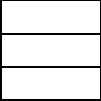
\includegraphics{resources/taskbook-99}\\Vista dall'alto}
		\hfill
		\parbox{0.2\linewidth}{\centering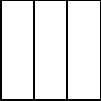
\includegraphics{resources/taskbook-98}\\Vista di fronte}
		\hfill\null
	\end{figure}
\end{problem}

\begin{problem}{15.}
	Quanti modi ci sono di ottenere il numero 64 come somma di dieci numeri naturali maggiori di 1, tra i quali il massimo sia 12?  [Modi che differiscono solamente per l’ordine degli addendi devono esser conteggiati una sola volta.]
\end{problem}

\begin{problem}{16.}
	Sovrapponendo poche sbarre simili una sull’altra (potrebbero essere per esempio tessere del domino) si può ottenere una sporgenza di lunghezza $x$. Qual è il massimo valore che si può ottenere per $x$?
	\begin{figure}
		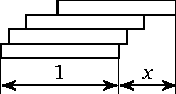
\includegraphics{resources/taskbook-97}
	\end{figure}
\end{problem}

\begin{problem}{17.}
	La distanza tra due città $A$ e $B$ è di \SI{40}{\km}. In uno stesso momento due ciclisti partono il primo da $A$ con una velocità di \SI{10}{\km\per\hour} e il secondo da $B$ con una velocità di  \SI{15}{\km\per\hour} e si muovono l'uno verso l'altro. Una mosca parte con il primo ciclista con una velocità di \SI{100}{\km\per\hour}, raggiunge il secondo, tocca la sua fronte e vola indietro verso il primo, tocca la sua fronte e torna verso il secondo e così via finché le fronti dei due ciclisti si scontrano e schiacciano la mosca. Quanti km ha fatto in tutto la mosca?
	\begin{figure}
		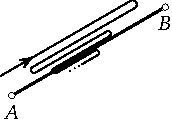
\includegraphics{resources/taskbook-1}
	\end{figure}
\end{problem}

\begin{problem}{18.}
	Una tessera del domino copre esattamente due quadrati di una scacchiera. Ricoprire con 31 pezzi del domino tutti i quadrati di una scacchiera  $8 \times 8$, tranne due che si trovino in due vertici opposti, come è illustrato nella figura.
	\begin{figure}
		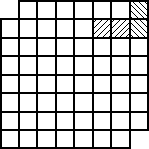
\includegraphics{resources/taskbook-2}
	\end{figure}
\end{problem}

\begin{problem}{19.}
	Nella stanza cubica disegnata qui sotto un bruco vuole strisciare dall' angoloindicato in basso a sinistra  all’angolo opposto indicato in alto a destra. Trovare il  percorso più breve lungo le pareti della stanza.
	\begin{figure}
		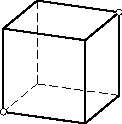
\includegraphics{resources/taskbook-3}
	\end{figure}
\end{problem}

\begin{problem}{20.}
	Si hanno due recipienti di volume 5~ litri e 3~ litri. Come si può, usando solamente questi due recipienti, ottenere esattamente un litro in uno di essi?
	\begin{figure}
		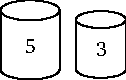
\includegraphics{resources/taskbook-4}
	\end{figure}
\end{problem}

\begin{problem}{21.}
	In una famiglia ci sono 5 teste e 14 gambe. Quante persone e quanti cani ci sono in quella famiglia?
\end{problem}

\begin{problem}{22.}
	Tre triangoli equilateri vengono costruiti esternamente sui lati $AB$, $BC$ e $CA$ di un triangolo $ABC$.
	Dimostrare che i loro centri ($*$) individuano un triangolo equilatero.
	\begin{figure}
		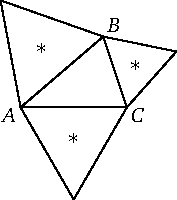
\includegraphics{resources/taskbook-6}
	\end{figure}
\end{problem}

\begin{problem}{23.}
	Quali poligoni si possono ottenere sezionando un cubo con un piano? Si può ottenere un pentagono? Un ettagono? E un esagono regolare?
	\begin{figure}
		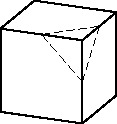
\includegraphics{resources/taskbook-7}
	\end{figure}
\end{problem}

\begin{problem}{24.}
	Tracciare una linea retta che passi per il centro di un cubo e sia tale che la somma dei quadrati delle distanze da essa degli otto vertici del cubo sia a) massima, b) minima (rispetto ad altre rette che  passano per il centro).
\end{problem}

\begin{problem}{25.}
	Un cono circolare retto viene tagliato da un piano lungo una curva chiusa. Due sfere inscritte nel cono sono tangenti al piano, una nel punto $A$ e l’ altra nel punto $B$. Trovare un punto $C$ sulla linea di taglio in modo che la somma delle distanze $CA + CB$ sia a) massima, b) minima.
	\begin{figure}
		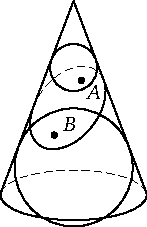
\includegraphics{resources/taskbook-9}
	\end{figure}
\end{problem}

\begin{problem}{26.}
	Si proietta la superficie della Terra sul cilindro formato dalle rette tangenti ai meridiani nel punto in cui intersecano l’equatore; la proiezione avviene lungo le semirette che sono parallele al piano dell’equatore e incidenti l’asse fra i due poli. L’area della proiezione della Francia sarà più grande o più piccola dell’area della stessa Francia?
	\begin{figure}
		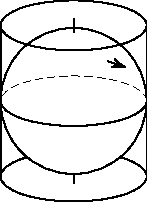
\includegraphics{resources/taskbook-10}
	\end{figure}
\end{problem}

\begin{problem}{27.}
	Dimostrare che, se $p$ è un primo dispari, il resto della divisione del numero  $2^{p-1}$ per $p$ è $1$.
	(Esempi: $2^2 = 3a + 1$, $2^4 = 5b+1$, $2^6 = 7c+1$, $2^{10} - 1 = 1023 = 11\cdot 93$)
\end{problem}

\begin{problem}{28.}
	Un ago lungo \SI{10}{\cm} viene gettato a caso su un foglio a righe in cui la distanza tra due righe vicine è pure di \SI{10}{\cm}. Questa azione viene ripetuta $N$ (un milione) di volte.
	Quante volte (approssimativamente, a meno di un errore percentualmente piccolo) l’ago caduto intersecherà una riga sul foglio?
	\begin{figure}
		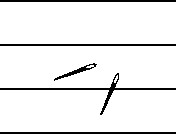
\includegraphics{resources/taskbook-12}
	\end{figure}
	Si può ripetere l’azione (come io feci all’età di 10 anni) con 100 invece che con un milione di lanci. [La risposta a questo problema è sorprendente:  $\frac2{\pi}N$. er un ago ricurvo di lunghezza $a \cdot \SI{10}{\cm}$ il numero di intersezioni che si osservano sarà approssimativamente $\frac{2a}{\pi}N$.
	Dove  $pi$ vale circa  $\pi \approx  \frac{355}{113} \approx \frac{22}7.$]
\end{problem}

\begin{problem}{29.}
	Tre tra i solidi platonici ci sono poliedri con facce triangolari: il tetraedro (4 facce), l’ottaedro (8 facce), l’icosaedro (20 facce -- è interessante provare a disegnarlo: esso ha 12 vertici e 30 spigoli).
	\begin{figure}
		\footnotesize
		\null\hfill
		\parbox{0.3\linewidth}{\centering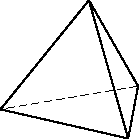
\includegraphics{resources/taskbook-131}\\Tetraedro($\text{tetra}= 4$)}
		\hfill
		\parbox{0.3\linewidth}{\centering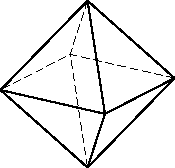
\includegraphics{resources/taskbook-132}\\Ottaedro ($\text{octo}= 8$)}
		\hfill\null\\
		{\Huge ?}\\Icosaedro
	\end{figure}
	È vero che per ogni poliedro di questo tipo (limitato, convesso con facce triangolari) il numero di facce è uguale a due volte il numero di vertici meno 4?


	Qui sotto un altro solido platonico (in tutto sono 5):
	\begin{figure}
		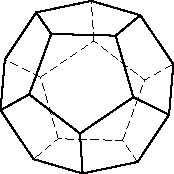
\includegraphics{resources/taskbook-14}
	\end{figure}
\end{problem}

\begin{problem}{30.}
	Un dodecaedro è un poliedro convesso con 12 facce che sono pentagoni regolari, 20 vertici e 30 spigoli (i suoi vertici sono i centri delle facce di un icosaedro).
Iscrivere in un dodecaedro 5 cubi (i vertici di ogni cubo devono essere vertici  del dodecaedro) i cui  spigoli siano diagonali delle facce del dodecaedro  (un cubo ha 12 ~spigoli, uno per ogni faccia). [Questa possibilità fu scoperta da Keplero nel corso dello studio sul moto dei pianeti.]
\end{problem}

\begin{problem}{31.}
	Trovare l’intersezione di due tetraedri iscritti in un cubo (in modo che i vertici di ciascuno siano vertici del cubo e gli spigoli siano diagonali delle facce). Quale frazione del volume del cubo è contenuta all’interno di tale intersezione?
\end{problem}

\begin{problem}{31\textsuperscript{bis}.}
	Tagliare un cubo mediante un piano che passi per tre punti fissatii sui suoi spigoli. [Disegnare il bordo del poligono ottenuto come intersezione del piano con le facce del cubo.]
	\begin{figure}
		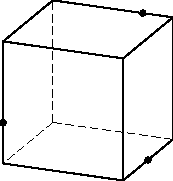
\includegraphics{resources/taskbook-15}
	\end{figure}
\end{problem}

\begin{problem}{32.}
	Quante simmetrie ha un tetraedro? Quante ne ha un cubo? E un ottaedro? E un icosaedro? E un dodecaedro? Una simmetria (di un poliedro) è una trasformazione che conserva le lunghezze (e che manda il poliedro in se stesso).
Quante sono le rotazioni e quante le riflessioni (in ciascuno dei cinque casi elencati)?
\end{problem}

\begin{problem}{33.}
	Quanti modi ci sono di colorare le $6$ facce di una serie di cubi con 6 colori [uno per faccia]  in modo che non ci siano due cubi colorati nello stesso modo(cioè due cubi che si possano ottenere l’uno dall’altro mediante una rotazione)?
	\begin{figure}
		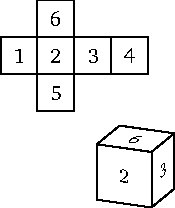
\includegraphics{resources/taskbook-17}
	\end{figure}
\end{problem}

\begin{problem}{34.}
	Quanti modi diversi ci sono di permutare $n$ oggetti?
	Per $n=3$ ce ne sono 6 : $(1,2,3)$, $(1,3,2)$, $(2,1,3)$, $(2,3,1)$, $(3,1,2)$, $(3,2,1)$. Per $n=4$? Per $n=5$? Per $n=6$? E per $n=10$?
	\begin{figure}
		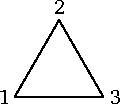
\includegraphics{resources/taskbook-18}
	\end{figure}
\end{problem}

\begin{problem}{35.}
	Un cubo ha $4$ diagonali da vertice a vertice. Quante permutazioni di questi 4 oggetti si ottengono mediante rotazioni del cubo stesso?
	\begin{figure}
		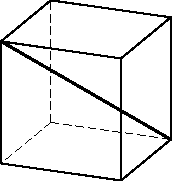
\includegraphics{resources/taskbook-19}
	\end{figure}
\end{problem}

\begin{problem}{36.}
È vero che la differenza tra il cubo della somma di tre interi e la somma dei cubi degli stessi numeri  è sempre divisibile per $3$?
\end{problem}

\begin{problem}{37.}
	Rispondere a una domanda analoga alla precedente, per le potenze quinte e la divisibilità per $5$ e poi per le potenze settime e la divisibilità per $7$.
\end{problem}

\begin{problem}{38.}
	Calcolare
	\begin{equation*}
		\frac{1}{1\cdot 2} + \frac{1}{2\cdot 3} + \frac{1}{3\cdot 4} + \dotsb + \frac{1}{99\cdot 100}
	\end{equation*}
	(con un errore non superiore all $1\%$).
\end{problem}

\begin{problem}{39.}
	Due poligoni con la stessa area, possono essere sempre scomposti in un numero finito di parti poligonali che si risistemano in modo da ottenere sia il primo poligono che il secondo. Dimostrarlo! [Per i solidi nello spazio tridimensionale questo non è più vero: un cubo e un tetraedro di ugual  volume non possono essere scomposti in parti con cui sia possibile ricostruire sia il cubo sia il tetraedro!]
	\begin{figure}
		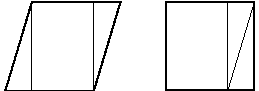
\includegraphics{resources/q39_horizontal}
	\end{figure}
\end{problem}

\begin{problem}{40.}
	Quattro vertici di un parallelogrammo sono stati scelti sugli incroci di un foglio di carta a quadretti in modo che né i lati del parallelogrammo né il suo interno contengano altri vertici della quadrettatura. Dimostrare che l’area di un tale parallelogrammo è uguale all’area di un quadretto.
	\begin{figure}
		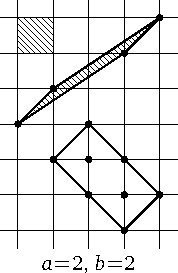
\includegraphics{resources/taskbook-24}
	\end{figure}
\end{problem}

\begin{problem}{41.}
	Trovare l’area di un parallelogrammo, con i vertici nei vertici di una quadrettatura come nel problema 40, che contenga $a$ vertici della quadrettatura all’interno e $b$ sui lati.
\end{problem}

\begin{problem}{42.}
	È vera anche per i parallelepipedi nello spazio tridimensionale l’affermazione contenuta nel quesito 40?
\end{problem}

\begin{problem}{43.}
	I numeri di Fibonacci costituiscono una successione $1,2,3,5,8,\allowbreak 13,21,34,\dotsc$, in cui $a_{n+2}=a_{n+1}+a_n$ per ogni
	$n=1,2,\dotsc$ ($a_n$ è l'$n$-esimo numero della successione). Trovare il massimo comun divisore tra i numeri $a_{100}$ e $a_{99}$.
\end{problem}

\begin{problem}{44.}
	Il numero (di Catalan) $c(n)$ rappresenta il numero di modi in cui  si può tagliare un poligono convesso di  $n$ lati in triangoli mediante diagonali che non si intersechino.
 Per esempio si ha $c(4)=2$, $c(5)=5$, $c(6)=14$. Come si può trovare $c(10)$?
	\begin{figure}
		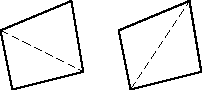
\includegraphics{resources/taskbook-281}
		\qquad
		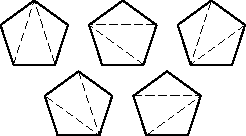
\includegraphics{resources/taskbook-282}
	\end{figure}
\end{problem}

\begin{problem}{45.}
	A un torneo di coppa partecipano $n$ squadre; ogni squadra perdente viene eliminata e la squadra vincitrice assoluta viene decisa dopo $n-1$ partite.
	Il programma dei tornei può essere scritto simbolicamente come, per esempio, $((a,(b,c)),d)$ per indicare che $b$ gioca contro $c$, che la squadra vincitrice gioca contro $a$, e che la squadra che vince  tra queste due si scontra con $d$.
	Qual è il numero delle diverse possibili programmazioni con 10 squadre?
	\begin{itemize}
		\item Per 2 squadre, abbiamo soltanto $(a,b)$, quindi questo numero è 1.
		\item Per 3 squadre, ci sono solo tre possibilità: $((a,b),c)$, o $((a,c),b)$, o $((b,c),a)$, e il numero è 3.
		\item Per 4 squadre:
			\begin{equation*}
				\begin{array}{@{}cccc@{}}
					(((a,b),c),d) & \quad\;(((a,c),b),d) & \quad\;(((a,d),b),c) & \quad\;(((b,c),a),d) \\
					(((b,d),a),c) & \quad\;(((c,d),a),b) & \quad\;(((a,b),d),c) & \quad\;(((a,c),d),b) \\
					(((a,d),c),b) & \quad\;(((b,c),d),a) & \quad\;(((b,d),c),a) & \quad\;(((c,d),b),a) \\
					((a,b),(c,d)) & \quad\;((a,c),(b,d)) & \quad\;((a,d),(b,c))
				\end{array}
			\end{equation*}
	\end{itemize}
\end{problem}

\begin{problem}{46.}
	Congiungere $n$ punti $1, 2, \dotsc, n$ tramite segmenti ($n-1$ in tutto) per ottenere un albero. Quanti diversi tipi di albero si possono ottenere? (Il caso $n=5$ è già interessante.)
	
	$n=2$:\quad 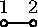
\includegraphics{resources/taskbook-291}\,,\quad il numero è1;

	$n=3$:\quad
	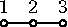
\includegraphics{resources/taskbook-292}\,,\quad
	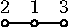
\includegraphics{resources/taskbook-293}\,,\quad
	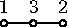
\includegraphics{resources/taskbook-294}\,,\quad
	 il numero è 3;

	$n=4$:\quad\def\quad{\hskip.7em}
	$\vcenter{\hbox{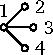
\includegraphics{resources/taskbook-295}}}$,\quad
	$\vcenter{\hbox{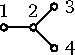
\includegraphics{resources/taskbook-296}}}$,\quad
	$\vcenter{\hbox{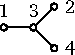
\includegraphics{resources/taskbook-297}}}$,\quad
	$\vcenter{\hbox{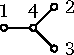
\includegraphics{resources/taskbook-298}}}$,\quad
	$\vcenter{\hbox{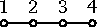
\includegraphics{resources/taskbook-299}}\hbox{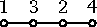
\includegraphics{resources/taskbook-290}}
	\vskip-8pt
	\hbox to50bp{\dotfill}}$,\\
	\null\hspace{\parindent}\phantom{$n=4$:}\quad  il numero è 16.
\end{problem}

\begin{problem}{47.}
	Una permutazione $(x_1,x_2, \dotsc,x_n)$ dei numeri $\{1, 2, \dotsc, n\}$ si chiama \emph{serpente} (di lunghezza $n$) se $x_1<x_2>x_3<x_4 \dotsb$.

	\begin{note}{Esempio:}
		\begin{equation*}
			\begin{aligned}[t]
				&\begin{aligned}[t] n=2, \text{\ \ soltanto\ \ } 1<2, \end{aligned} &&\text{il numero dei possibili serpenti è }1, \\
				&\hskip-\nulldelimiterspace\mathord{\left.\begin{aligned} n=3, \hphantom{\text{\ \ only\ \ }} 1&<3>2 \\
				2&<3>1\end{aligned} \right\}}, && \text{il numero è }2, \\
				&\hskip-\nulldelimiterspace\mathord{\left.\begin{aligned} n=4, \hphantom{\text{\ \ only\ \ }} 1&<3>2<4 \\
				1&<4>2<3 \\
				2&<3>1<4 \\
				2&<4>1<3 \\
				3&<4>1<2\end{aligned} \right\}},
				&&\text{il numero è }5. \\
			\end{aligned}
		\end{equation*}
	\end{note}
	Trovare il numero di serpenti di lunghezza  $10$.
\end{problem}

\begin{problem}{48.}
	Sia $s_n$ il numero di serpenti di lunghezza $n$:
	\begin{equation*}
		s_1=1, \quad s_2=1, \quad s_3=2, \quad s_4=5, \quad s_5=16, \quad s_6=61.
	\end{equation*}
	Dimostrare che la serie di Taylor della tangente è
	\begin{equation*}
		\tan x=1\, \frac{x^1}{1!}+2\, \frac{x^3}{3!}+16\, \frac{x^5}{5!}+\dots=
		\textstyle\sum\limits_{k=1}^{\infty} s_{2k-1}\, \frac{x^{2k-1}}{(2k-1)!}.
	\end{equation*}
\end{problem}

\begin{problem}{49.}
	Trovare la somma della serie
	\begin{equation*}
		1+1\, \frac{x^2}{2!}+5\, \frac{x^4}{4!}+61\, \frac{x^6}{6!}+\dots=
		\textstyle\sum\limits_{k=0}^{\infty} s_{2k}\,\frac{x^{2k}}{(2k)!}.
	\end{equation*}
\end{problem}

\begin{problem}{50.}
	Per $s>1$, dimostrare l’identità:
	\begin{equation*}
		\textstyle\prod\limits_{p=2}^{\infty} \frac{1}{1-\frac{1}{p^s}}=\textstyle\sum\limits_{n=1}^{\infty} \frac{1}{n^s}.
	\end{equation*}
	(dove il prodotto è su tutti i numeri primi $p$ e la somma è su tutti i numeri naturali ~$n$).
\end{problem}

\begin{problem}{51.}
	Trovare la somma della serie:
	\begin{equation*}
		1+ \frac{1}{4}+ \frac{1}{9}+\dots=\textstyle\sum\limits_{n=1}^{\infty} \frac{1}{n^2}.
	\end{equation*}
	[Dimostrare che la somma è uguale a $\nicefrac{\pi^2}{6}$, che è approssimativamente  $\nicefrac{3}{2}$.]
\end{problem}

\begin{problem}{52.}
	Trovare la probabilità che la frazione  $\nicefrac{p}{q}$ sia irriducibile (in base alla seguente definizione:
	nel disco $p^2+q^2 \leqslant R^2$, considerate il numero $N$ of di punti a coordinate intere $p$ e $q$ che non abbiano un divisore comune maggiore di 1; e chiamate probabilità che una certa frazione $\nicefrac{p}{q}$ sia irriducibile il limite del rapporto $\nicefrac{N(R)}{M(R)}$, dove $M(R)$ è il numero di punti a coordinate intere nel disco $(M \sim \pi R^2)$).
	\begin{figure}
		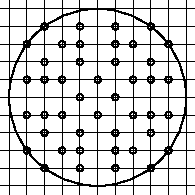
\includegraphics{resources/taskbook-36}\\
		\footnotesize $M(5)=81$, $N(5)=44$, $\nicefrac{N}{M} = \nicefrac{44}{81}$
	\end{figure}
\end{problem}

\begin{problem}{53.}
	Per la successione di Fibonacci (vedi problema 43), trovare il limite del rapporto
	$a_{n+1}/a_n$ quando $n$ tende all’infinito:\vspace{2\jot}
	\begin{equation*}
		\frac{a_{n+1}}{a_n}=2,\ \frac 32,\ \frac53, \ \frac85, \ \frac{13}8,
		\ \frac{34}{21}.
	\end{equation*}
	[RISPOSTA: tale limite è il \enquote{rapporto aureo},
	$\frac{\sqrt{5}+1}{2\vphantom)} \approx 1.618$. Si tratta del rapporto tra i lati di un foglio rettangolare che rimane simile a se stesso dopo avere tagliato via un quadrato di lato uguale al lato minore del rettangolo,
	$\frac{AB}{BC}=\frac{PC}{CD}$. Come è legato il rapporto aureo al pentagono regolare e alla stella a cinque punte?
	\begin{figure}
		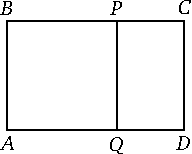
\includegraphics{resources/taskbook-37}
	\end{figure}
\end{problem}

\begin{problem}{54.}
Calcolare la frazione continua e infinita
	\begin{equation*}
		1+\cfrac{1}{2+\cfrac{1}{1+\cfrac{1}{2+\cfrac{1}{1+\cfrac{1}{2+\ldots}}}}}=
		a_0+\cfrac{1}{a_1+\cfrac{1}{a_2+\cfrac{1}{a_3+\dots}}}
	\end{equation*}
	con $a_{2k}=1$ e $a_{2k+1}=2$ (si tratta dunque di trovare il limite della frazione
	\begin{equation*}
		a_0+\cfrac{1}{a_1+\cfrac{1}{a_2+{\atop{\ddots \atop {}} + \cfrac{1}{a_n}}}}
	\end{equation*}
	per $n \to \infty$).
\end{problem}

\begin{problem}{55.}
	Trovare i polinomi y=p(x)
	\begin{equation*}
		y=\cos 3 (\arccos x),\ y=\cos 4 (\arccos x),\
		y=\cos n (\arccos x),
	\end{equation*}
	dove $|x| \leqslant 1$.
\end{problem}

\begin{problem}{56.}
	Calcolare la somma delle potenze $k$-esime delle $n$ radici complesse $n$-esime dell'unità.
\end{problem}

\begin{problem}{57.}
Sul piano $(x,y)$, tracciare le curve definite parametricamente da:
	\begin{equation*}
		\{x=\cos 2t, y=\sin 3t\},\quad
		\{x=t^3-3t, y=t^4-2t^2\}.
	\end{equation*}
	\vspace{-2\baselineskip}%remove this vertical space if your translation has text coming after the equation
\end{problem}

\begin{problem}{58.}
	Calcolare (con un errore di non più del 10\%)
 $\int_0^{2\pi} \sin^{100} x\,dx$ .
\end{problem}

\begin{problem}{59.}
	Calcolare (con un errore di non più del 10\%)  $\int_1^{10} x^x\,dx$ .
\end{problem}

\begin{problem}{60.}
	Su una superficie sferica di raggio unitario, trovare l’area di un triangolo di angoli $(\alpha, \beta, \gamma)$ i cui lati siano archi di circonferenze massime.

	\begin{note}{RISPOSTA:}
		$S=\alpha+\beta+\gamma-\pi$ (per un triangolo con tre angoli retti  $S=\nicefrac{\pi}{2}$, ovvero un ottavo dell’area totale della sfera).
		\begin{figure}
			\null\hfill
			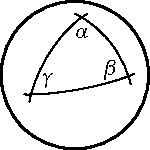
\includegraphics{resources/taskbook-44}
			\hfill
			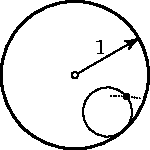
\includegraphics{resources/taskbook-45}
			\hfill\null
		\end{figure}
	\end{note}
\end{problem}

\begin{problem}{61.}
	Un cerchio di raggio $r$ rotola senza strisciare all’interno di un cerchio di raggio  1.
	Tracciare la traiettoria percorsa da un punto del cerchio che rotola (questa traiettoria si chiama ipocicloide) per $r=\nicefrac{1}{3}$, per $r=\nicefrac{1}{4}$, per $r=\nicefrac{1}{n}$, e per $r=\nicefrac{1}{2}$.
\end{problem}

\begin{problem}{62.}
	Stimare la probabilità che in una classe di $n$ alunni ce ne siano due che compiono gli anni nello stesso giorno. E’ alta o bassa?

	\begin{note}{RISPOSTA:}
		È (molto) alta se il numero di alunni è (ben) al di sopra di $n_0$,
		(molto) bassa se il numero di alunni è (ben) al di sotto di  $n_0$. E occorre stimare questo valore  $n_0$
		(corrispondente a una probabilità $p \approx \nicefrac{1}{2}$).
	\end{note}
\end{problem}

\begin{problem}{63.}
	La legge di Snell (o di Snellius) stabilisce che l’angolo  $\alpha$ formato da un raggio di luce con la normale agli strati di un mezzo stratificato soddisfa l’equazione
	\begin{equation*}
		n(y) \sin \alpha=\text{costante},
	\end{equation*}
	dove $n(y)$ è l’indice di rifrazione dello strato all’altezza $y$ (il valore $n$ è inversamente proporzionale alla velocità della luce nel mezzo assumendo uguale a 1 la velocità della luce nel vuoto; nell’acqua, in particolare $n=\nicefrac{4}{3}$).
	\begin{figure}
		\null\hfill
		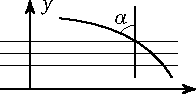
\includegraphics{resources/taskbook-47}
		\hfill
		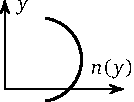
\includegraphics{resources/taskbook-471}
		\hfill\null
	\end{figure}

	Disegnare le traiettorie dei raggi nel mezzo  \enquote{aria sopra un deserto}, dove l'indice $n(y)$ raggiunge il massimo a una certa altezza. (Una soluzione a questo problema spiega i miraggi nel deserto per chi ha già chiaro come le traiettorie dei raggi che provengono dagli oggetti sono collegate alle loro immagini.)
\end{problem}

\begin{problem}{64.}
	 Iscrivere in un triangolo acutangolo $ABC$ un triangolo $KLM$ di perimetro minimo
	(con il vertice $K$ sul lato $AB$, $L$ su $BC$ e $M$ su $CA$).
	\begin{figure}
		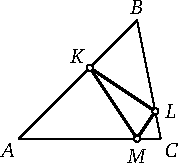
\includegraphics{resources/taskbook-48}
	\end{figure}

	\begin{note}{Suggerimento:}
		La risposta per triangoli non acutangoli è ben diversa dalla bella risposta che si ottiene per i triangoli acutangoli.
	\end{note}
\end{problem}

\begin{problem}{65.}
	Calcolare il valor medio della funzione $\nicefrac{1}{r}$ (dove
	$r^2=x^2+y^2+z^2$, e $r$ è la distanza dall’origine) nella sfera di raggio
	$R$ centrata nel generico punto $(X,Y,Z)$.

	\begin{note}{Suggerimento:}
 questo problema è collegato alla legge di gravitazione di Newton e alla legge di interazione elettrica di Coulomb. Nella versione bidimensionale del problema la funzione dovrebbe essere sostituita da $\ln r$, e la sfera dal cerchio.
	\end{note}
\end{problem}

\begin{problem}{66.}
	Il fatto che sia $2^{10}=1024 \approx 10^3$ implica che
	$\log_{10} 2 \approx 0.3$. Stimare di quanto questi due valori differiscono e calcolare $\log_{10} 2$  alla terza cifra decimale.
\end{problem}

\begin{problem}{67.}
	Trovare $\log_{10} 4$, $\log_{10} 8$,
	$\log_{10} 5$, $\log_{10} 50$, $\log_{10} 32$, $\log_{10} 128$,
	$\log_{10} 125$, $\log_{10} 64$ con lo stesso livello di precisione.
\end{problem}

\begin{problem}{68.}
	Usando il fatto che $7^2 \approx 50$, trovare un valore approssimato del $\log_{10} 7$.
\end{problem}

\begin{problem}{69.}
	Conoscendo $\log_{10} 64$ e $\log_{10} 7$, trovare $\log_{10} 9$, $\log_{10} 3$,
    $\log_{10} 27$, $\log_{10} 6$, $\log_{10} 12$.
\end{problem}

\begin{problem}{70.}
	Usando il fatto che $\ln (1+x) \approx x$ ( dove $\ln$ è $\log_e$), trovare $\log_{10} e$ e
    $\ln 10$ dalla relazione\footnote{Il numerodi Eulero $e = 2{.}71828\dots$ si definisce come il limite della successione
	$\left(1+\frac{1}{n}\right)^n$ per $n\to \infty$, ed è uguale alla somma della serie
	$1+\frac{1}{1!} +\frac{1}{2!}+\frac{1}{3!}+\dotsb$. Si può anche definire attraverso la  formula citata per $\ln (1+x)$: $\lim\limits_{x\to 0}\frac{\ln(1+x)}{x} = 1$.}
	%
	\begin{equation*}
		\log_{10} a=\frac{\ln a}{\ln 10}
	\end{equation*}
	e dai valori di $\log_{10} a$ calcolati precedentemente (per esempio, per $a=128/125, 1024/1000$
	e così via).

	[Le soluzioni ai problemi dal  65 al 69 forniscono in mezz’ora una tabella di logaritmi con la precisione di quattro cifre decimali per qualsiasi numero usando il prodotto di numeri per i quali si sono già trovati i logaritmi e la formula
	\begin{equation*}
		\ln (1+x) \approx x-\frac{x^2}{2}+\frac{x^3}{3}-\frac{x^4}{4}+\dotsb,
	\end{equation*}
	per le correzioni.] (In  questo modo Newton compilò una tavola di logaritmi a 40 cifre decimali!)
\end{problem}

\begin{problem}{71.}
	Considerare la  successione delle potenze di $2$: $1$, $2$, $4$, $8$, $16$, $32$, $64$,
	$128$, $256$, $512$, $1024$, $2048, \dotsc$ Tra i primi dodici numeri quattro hanno una scrittura in base 10 che inizia con la cifra 1, e nessuno di essi comincia con la cifra 7.

	Dimostrare che per $n \to \infty$ la frequenza $p_{k}$ con cui appare k come prima cifra del numero $2^m$, essendo
	$0\leqslant m \leqslant n$, è:
	$p_1 \approx 30\%, p_2 \approx 18\%, \dotsc, p_9 \approx 4\%$.
\end{problem}

\begin{problem}{72.}
	Verificare il comportamento delle prime cifre delle potenze di 3: $1,
	3, 9, 2, 8, 2, 7, \dotsc$ Dimostrare che, anche in questo caso, per $n \to \infty$
si ottengono certe frequenze $p_{k}$ con cui appare k come prima cifra del numero  $3^m$, con
	$0\leqslant m \leqslant n$, e esse sono, per di più, le stesse frequenze che troviamo per le potenze di 2. Trovare una formula esatta per $p_1, \dotsc, p_9$.

	\begin{note}{SUGGERIMENTO:}
		La prima cifra di un numero $x$ è determinata dalla parte frazionaria del numero $\log_{10} x$, perciò occorre considerare la successione delle parti frazionarie del numero          $m \alpha$ con $\alpha=\log_{10} 2$.
	\end{note}
	Dimostrare che queste parti frazionarie sono distribuite uniformemente nell’intervallo da 0 a~1: delle $n$ parti frazionarie dei numeri $m \alpha$, $0 \leqslant m<n$,
	un sottointervallo $A$ conterrà la quantità ~$k_n (A)$ in modo che, per $n \to \infty$,
	$\lim (k_n (A)/n)=(\text{lunghezza del sottointervallo ~$A$})$.
\end{problem}

\begin{problem}{73.}
	Sia $g\colon M \to M$ una mappa liscia da un dominio limitato $M$ in se stesso che sia biunivoca e conservi le aree (volumi nel caso multi dimensionale) dei domini.

	Dimostrare che in ogni intorno $U$ di un qualsiasi punto di $M$ e per ogni $N$ esiste un punto $x$
	tale che anche $g^T x$ appartiene ad $U$ per un certo intero $T>N$ (\enquote{teorema della ricorrenza}).
\end{problem}

\begin{problem}{74.}
	Sia $M$ la superficie di un toro (con coordinate $\alpha \pmod{2\pi}$, $\beta \pmod{2\pi}$),
	e
	\begin{equation*}
		g(\alpha, \beta)=(\alpha+1, \beta+ \sqrt{2}) \pmod{2\pi}.
	\end{equation*}
	Dimostrare che la successione di punti
	$\{g^T (x)\}$, $T=1, 2, \dotsc$, è ovunque densa sul toro.
\end{problem}

\begin{problem}{75.}
	Con la notazione del problema 74, sia
	\begin{equation*}
		f(\alpha, \beta)=(2\alpha+\beta,\alpha+\beta) \pmod{2\pi}.
	\end{equation*}
	Dimostrare che esiste un sottoinsieme del toro ovunque denso che consiste di punti periodici  $x$ (cioè tali che
	$f^{T (x)} x=x$ per un certo intero $T>0$).
\end{problem}

\begin{problem}{76.}
	Con le notazioni del problema 74 dimostrare che per quasi tutti i punti $x$ del toro, la successione di punti  $\{g^T (x)\}$, $T=1, 2, \dotsc$, è ovunque densa sul toro
	(i punti $x$ che non godono di questa proprietà costituiscono un insieme di misura nulla).
\end{problem}

\begin{problem}{77.}
	Nei problemi 74 e 76 dimostrare che la successione  $\{g^T (x)\}$, $T=1, 2, \dotsc$, è distribuita sul toro uniformemente: se un dominio $A$ contiene $k_n(A)$ punti fra gli $n$ che si ottengono per $T=1, 2, \dotsc,n$, allora
	\begin{equation*}
		\lim_{n \to \infty} \frac{k_n(A)}{n}=\frac{\operatorname{mis} A}{\operatorname{mis} M}
	\end{equation*}
	(per esempio, per un dominio di Jordan misurabile $A$ di misura $\operatorname{mis} A$).
\end{problem}

\null\vfill
\begin{note}{Un'osservazione al problema 13.}
	Ho cercato di illustrare con questo problema, la differenza di approccio ai problemi tra un matematico e un fisico, in un mio articolo su invito nella rivista \enquote{Physics -- Uspekhi} in occasione del Natale del 2000. Il successo ha superato di gran lunga le mie intenzioni: l’editore, a differenza dei bambini in età prescolare sui quali avevo basato i miei esperimenti,
non è riuscito a risolvere il problema e per questo lo ha modificato nel modo seguente, in modo che si accordasse con la mia risposta di \SI{4}{\mm}: invece di scrivere \enquote{dalla prima paginadel volume 1 all'ultima pagina del volume 2} ha scritto \enquote{dall' \emph{ultima} pagina del volume 1 alla \emph{prima} pagina del volume 2}.

	Questa storia vera è talmente inverosimile che la includo qui: la prova di quanto è accaduto sta nella versione pubblicata dall’editore sulla rivista.
\end{note}
\clearpage
\null\vfill
\noindent
Traduzione Russo-Inglese:\\
\null\quad Victor Goryunov e Sabir Gusein-Zade\\
\\
\noindent
Traduzione Inglese-Italiano:\\
\null\quad Donatella De Tommaso\\
\\
Disegni e impaginazione:\\
\null\quad Konrad Renner and Christian Stussak\\
\\
\\
Dall'edizione Russa:\\
\null\quad \textrussian{В. И. Арнольд: Задачи для детей от 5 до 15 лет}\\
\null\quad Moscow, MCCME, 2004\\
\null\quad ISBN 5-94057-183-2\\
\\
\\
Crediti delle immagini alla pagina:\\
\null\quad Archivio dell'Istituto di Ricerca Matematica Oberwolfach\\
\\
Versione:\\
\null\quad \today\\
\\
Questo libro è coperto da licenza CC BY-NC-SA 3.0 sulla piattaforma IMAG\-I\-NARY: \href{http://www.imaginary.org/background-materials}{www.imaginary.org/background-materials}.\\
IMAGINARY è un progetto dell'Istituto di Ricerca Matematica Oberwolfach sostenuto dalla Fondazione Klaus Tschira.
\end{document}
